% Autor šablony: Jakub Dokulil (kubadokulil99@gmail.com) https://github.com/Kubiczek36/SOC_sablona

\documentclass[12pt, a4paper,
  %oneside,      %% -- odkomentujte, pokud chcete svou práci mít pouze jednostrannou, mezera pro hřbet pak automaticky bude pouze na levé straně
 twoside,        %% -- pro oboustranné práce, mezera pro hřbet následně střídá strany.
 openright
]{report}

%% Nutné balíčky a nastavení
%%%%%%%%%%%%%%%%%%%%%%%%%%%%

\newcommand\city{Pardubice} 
\newcommand\district{Pardubický}
\newcommand\specialization{Obor č. 18: Informatika}
\newcommand\school{SŠIE Delta}
\newcommand\consultant{RNDr. Koupil Jan, Ph.D.}
\newcommand\name{Krátký Kryštof}
\newcommand\publicationYear{2022}

\title{Histories} %% -- Název tvé práce
\author{\name} %% -- tvé jméno
\date{\publicationYear} %% -- rok, kdy píšeš SOČku

\usepackage[top=2.5cm, bottom=2.5cm, left=3.5cm, right=1.5cm]{geometry} %% nastaví okraje, left -- vnitřní okraj, right -- vnější okraj

\usepackage[czech]{babel} %% balík babel pro sazbu v češtině
\usepackage[utf8]{inputenc} %% balíky pro kódování textu m
\usepackage[T1]{fontenc}
\usepackage{cmap} %% balíček zajišťující, že vytvořené PDF bude prohledávatelné a kopírovatelné

\usepackage{graphicx} %% balík pro vkládání obrázků

\usepackage{subcaption} %% balíček pro vkládání podobrázků

\usepackage{hyperref} %% balíček, který v PDF vytváří odkazy

\linespread{1.15} %% řádkování

\usepackage[pagestyles]{titlesec} %% balíček pro úpravu stylu kapitol a sekcí
\titleformat{\chapter}[block]{\scshape\bfseries\LARGE}{\thechapter}{10pt}{\vspace{0pt}}[\vspace{-22pt}]
\titleformat{\section}[block]{\scshape\bfseries\Large}{\thesection}{10pt}{\vspace{0pt}}
\titleformat{\subsection}[block]{\bfseries\large}{\thesubsection}{10pt}{\vspace{0pt}}

\setcounter{secnumdepth}{2}
\setcounter{tocdepth}{1}
\usepackage{fancyhdr}
\pagestyle{fancy}
\renewcommand{\headrulewidth}{1pt}

\newenvironment{propertiesItemize}{
\begin{itemize}{ 
  }}
  {\end{itemize}}

\usepackage{booktabs}

\usepackage{url}

%% Balíčky co se můžou hodit :) 
%%%%%%%%%%%%%%%%%%%%%%%%%%%%%%%

\usepackage{pdfpages} %% Balíček umožňující vkládat stránky z PDF souborů, 

\usepackage{upgreek} %% Balíček pro sazbu stojatých řeckých písmen, třeba u jednotky mikrometr. Například stojaté mí: \upmu, stojaté pí: \uppi

\usepackage{amsmath}    %% Balíčky amsmath a amsfonts 
\usepackage{amsfonts}   %% pro sazbu matematických symbolů
\usepackage{esint}     %% pro sazbu různých integrálů (např \oiint)
\usepackage{mathrsfs}

%% makra pro sazbu matematiky
\newcommand{\dif}{\mathrm{d}} %% makro pro sazbu diferenciálu, místo toho
%% abych musel psát '\mathrm{d}' mi stačí napsat '\dif' což je mnohem 
%% kratší a mohu si tak usnadnit práci

%% Bordel pro práci - můžeš smáznout :) 
%%%%%%%%%%%%%%%%%%%

\usepackage{lipsum} %% balíček který píše lipsum (nesmyslný text, který se používá pro kontrolu typografie)

%% Začátek dokumentu
%%%%%%%%%%%%%%%%%%%%


\begin{document}

\pagestyle{empty}
\pagenumbering{Roman}


\begin{titlepage}
    \bfseries{ %%% písmo na stránce je tučně
        \begin{center}
            \LARGE{STŘEDOŠKOLSKÁ ODBORNÁ ČINNOST} 
            \vspace{14pt}
            \large{\specialization} 

            \vspace{0.4 \textheight}

            \LARGE{ %%%%
                Histories
            }%%%%

            \vspace{0.4\textheight}
        \end{center}
        
        \noindent\Large{\name}

        \noindent\Large{\district\hspace{\stretch{1}}  \city, \publicationYear} %% vyplň oficiální název kraje, město a rok
        
            
    } %%%
\end{titlepage}

\cleardoublepage%% Úvodní stránka s informacemi
{\bfseries %%% písmo na stránce je tučně
    \begin{center}
        \LARGE{STŘEDOŠKOLSKÁ ODBORNÁ ČINNOST}

        \vspace{14pt}
        {\large \specialization}

        \vspace{0.3 \textheight}

        \LARGE{ %%%%
        Histories
        }

        \LARGE{ %%%%
        platforma pro sdílení historických fotek
        }%%%%

        \vspace{0.24\textheight}
    \end{center}  
}%%%
{\Large %%%
    \noindent\textbf{Jméno:} \name\\
    \textbf{Škola:} \school\\
    \textbf{Kraj:} \district\\
    \textbf{Konzultant:} \consultant\\
} %%%

\noindent \city, \publicationYear\cleardoublepage\noindent{\Large{\bfseries{Prohlášení}}}  %% uprav si koncovky podle toho na jaký rod se cítíš, vypadá to pak lépe :) 

\noindent Prohlašuji, že jsem svou práci SOČ vypracoval/a samostatně a použil/a jsem pouze prameny a literaturu uvedené v seznamu bibliografických záznamů.

\noindent Prohlašuji, že tištěná verze a elektronická verze soutěžní práce SOČ jsou shodné. 

\noindent Nemám závažný důvod proti zpřístupňování této práce v souladu se zákonem č. 121/2000 Sb., o právu autorském, o právech souvisejících s právem autorským a o změně některých zákonů (autorský zákon) ve znění pozdějších předpisů. 

\vspace{24 pt}

\noindent V Pardubicích dne 9.\ září 2022 \dotfill{}\hspace{\stretch{0.5}} 

\hspace{8cm} \name\cleardoublepage\vspace*{0.8\textheight}
\noindent{\Large{\bfseries{Poděkování}}}

\noindent
Rád bych poděkoval svému konzultantovi RNDr. Janu Koupilovi, Ph.D. za odborné vedení a konzultace při tvorbě tohoto projekt.

\cleardoublepage\noindent{\Large{\bfseries{Abstrakt}}}

\noindent TBD abstrakt

\vspace{18pt}

\noindent{\Large{\bfseries{Klíčová slova}}}

\noindent Webová aplikace; sociální síť; sdílení historických fotek

\vspace{18pt}

\noindent{\Large{\bfseries{Abstract}}}

\noindent TBD abstract

\vspace{18pt}

\noindent{\Large{\bfseries{Keywords}}}

\noindent Web app; social media; historical photo sharing

\cleardoublepage\tableofcontents

\pagenumbering{arabic}
\pagestyle{fancy}
\setcounter{page}{1}


\chapter{Pojmy}
\subsection{NSFW}
Zkratka vycházející z anglického "Not Safe For Work" (nevhodné pro práci), zpravidla se takto označují příspěvky obsahující nahotu, násilí a tudíž by se jim mělo vyhnout v profesionálním prostředí. \cite{NSFW}

\subsection{Garbage collection} je správa paměti, Stará se o uvolnění nepoužívaných úseků v paměti které nejsou procesem využívány \cite{GarbageCollection}

\subsection{Runtime environment} je skupina software umožňující spuštění programu v reálném čase, obvykle implementuje základních funkce jako je například výpis textu nebo připojení k internetu \cite{whatIsRuntimeEnvironment}


\chapter{Úvod}
\section{Cíl}
Cílem projektu bylo vytvořit platformu pro sdílení historických fotografií
s informací o místě a čase pořízení. Jednou z hlavních funkcí aplikace je možnost
zobrazení fotografií na mapě včetně možnosti filtrování podle časové osy. Prohlížet 
příspěvky mají možnost všichni včetně neregistrovaných uživatelů. Registrovaní 
uživatelé dále mohou přidávat nové příspěvky a diskutovat s ostatními uživateli v
komentářové sekci. Zároveň existují administrátorské funkce, které umožňují mazat
nevhodný obsah a přidávat detaily míst (např. název místa, fotku, ikonu na mapě, atd.).

\section{Motivace}
Motivací projektu byla Facebooková skupina Pardubice v běhu času\cite{PardubiceVBehuCasuFB}, kde lidé 
sdílí historické fotky. Na rozdíl od Histories zde není téměř žádná možnost filtrování či 
řazení ani zobrazení příspěvků na mapě.




\section{Existující řešení}
\subsection{Historypin}
Historypin je open-source platforma fungující jako archiv historických fotografií.Umožňuje vyhledávání míst na mapě, filtrování příspěvků podle data vzniku, nebo například vytváření kolekcí. Obashuje velké množství příspěvků, což ale vede k pomalému načítání stránky a dat na mapě. Zvolený layout snižuje přehlednost a zhoršuje orientaci a navigaci na stránce.
\subsection{Facebook}
Primární účel Facebooku je sdílení aktuálních příspěvků. Neobsahuje téměř žádné možnosti filtrování či geolokaci příspěvků. 

\chapter{Použité technologie}
\section{Sdílené technologie pro frontend i backend}
\subsection{Typescript}
Typescript je nadstavba na Javascript, která umožňuje statické typování \cite{DynamicVsStaticTyping}. Všechen kód napsaný v Javascriptu je validním také v Typescriptu. \cite{whatIsTypescript}\cite{typescriptForTheNewProgrammer}
\subsection{NPM}
NPM je nástroj pro správu Javascript knihoven. Umožňuje jednoduchou instalaci knihoven použitých v projektu. V konfiguračním souboru lze nastavit nutnost použití konkrétní verze knihovny, což zajišťuje stejnou funkčnost napříč různými zařízeními. \cite{whatIsNpmW3}\cite{aboutNpm}
\subsection{GraphQL}
GraphQL je dotazovací jazyk pro API \cite{graphqlIntroduction}. Nejpoužívanější alternativou pro GraphQL je REST. Oproti REST je u GraphQL výhodou že klient v requestu specifikuje data která chce aby byla vrácena ze serveru. Tímto je eliminován přenos nepotřebných dat a tím také celý přenos urychlen. Zároveň se klient dotazuje vždy na stejný endpoint, mění se pouze obsah requestu. GraphQL je typované \cite{graphqlTypes}, což znamená že musí být předem jasné typ vrácených dat. \cite{restApiRedHat}\cite{whatIsApiAws}


% FRONTEND %%%%%%% 
\section{Technologie pro frontend}
\subsection{React}
React je Javascriptová knihovna pro tvorbu webových stránek zjednodušující práci s měnícími se daty. Kód je dělen na jednotlivé celky nazývané komponenty \cite{reactComponentsAndProps}. Komponenty mohou být v kódu používány vícekrát, což vede k zjednodušení a zefektivnění psaní kódu. \cite{gettingStartedReact}
\subsection{Next.js}
Next.js je React framework zaměřený na zlepšení uživatelské i vývojářské zkušenosti. Hlavní výhodou Next.js je server side rendering \cite{whatIsSSR}, což znamená že se data načtou již na serveru a klientovi se posílá načtená stránka, na rozdíl od klasického Reactu, kde se klientovi pošle prázdná stránka a až poté se u klienta načítají data. Server side rendering zároveň zlepšuje skóre SEO \cite{whatIsSEO}. Next.js disponuje vlastními React komponenty, například Link, který zajišťuje prefetchování odkazů, nebo Image, který optimalizuje způsob načítání obrázků. Next.js obsahuje také file system rounting, což znamená že není nutné nastavovat React router. \cite{nextGetStarted}
\subsection{Tailwind}
Tailwind je open-source CSS framework, který umožňuje rychlejší a přehlednější psaní stylů stránek pomocí předvytvořených tříd. Tailwind neobsahuje žádné předvytvořené prvky.\cite{tailwindDocumentation}
\subsection{GraphQL code generator}
GraphQL code generator je knihovna, která umožňuje generování Typescript typů z GraphQL schématu. Díky tomu není nutné vytvářet zvlášť nové typy pro GraphQL response. \cite{graphqlCodeGeneratorDocs}
% BACKEND %%%%%%% 
\section{tachnologie pro backend}
\subsection{Nodejs}
Node js je runtime environment pro spouštění Javascriptu mimo prohlížeč. Hlavním důvodem pro použití bylo použití stejného programovacího jazyka pro backend i frontend, což umožňuje opakované využívání některých funkcí (např. validace). \cite{aboutNodeJS}
 
\chapter{Úložiště dat}
    \section{Úložiště souborů}
        \subsection{Protokol IPFS}\label{subsection:IPFS}
        Inter Planetary File System (Meziplanetární souborový systém) je peer-to-peer trustless protokol pro ukládání a sdílení souborů v distribuovaném souborovém systému. \cite{IPFSDocs}
        \subsubsection{Decentralizace}
            Decentralizované protokoly nemají vlastníka a jsou utvářeny všemi uživateli společně. Tento koncept často bývá spojen s konceptem trustless, který umožňuje každému uživateli kdykoliv ověřit pravdivost obsahu, v tomto případě vygenerováním hashe a následným porovnáním dvou hashů, čímž je zabráňeno cenzuře \cite{decentralizedVsTrustless}. Decentralizace umožňuje rychlejší načtení obsahu, pokud je v blízkosti node s uloženým obsahem, nebo načtení obsahu bez nutnosti přístupu k celosvětové síti, pokud je v lokální síti node, který obsah poskytuje. \cite{decentralizedAndDistributedNetworks}\cite{decentralizedAndTrustless}
        \subsubsection{Zpracování obsahu}
            \paragraph{Nahrávání obshu}
            Při ukládání souboru do IPFS je pomocí algoritmu sha-256 z obsahu souboru vygenerován hash, který slouží jako unikátní identifikátor souboru (CID) pomocí kterého je následně soubor přístupný \cite{IPFScontentAddressing}. Vygenerovaný hash má vždy stejnou délku nezávisle na velikosti daného souboru a při nahrání souboru se shodným obsahem z jakéhokoliv zařízení bude vždy hash totožný, čímž je zajištěna neměnnost obsahu. Nahrané soubory si můžou jednotlivé nody připnout, což je ochrání před garbage collection \cite{IPFSPersistence}. Po připnutí je soubor uložen do úložiště nodu a dál poskytován síti. Existují tzv. pinning services, které umožňují pronajmutí nodu, s přístupem k vysokorychlostnímu internetu a je spravován poskytovatelem. V projektu byl použit pinning service Infura. 
            \paragraph{Přístup k obsahu} K obsahu je následně možné přistupovat skrz veřejnou gateway (např. ipfs.io, nebo cf-ipfs.com), nebo skrz gateway nodu, kde jsou připnuté soubory, díky čemuž není nutné vyhledávat nejbližší node poskytující obsah, což celý proces urychluje. \cite{IPFSgateways}
        \subsection{Porovnání IPFS a S3}
            Soubory v IPFS jsou adresovány na základě obsahu na rozdíl od S3, kde jsou sobory adresovány na základě lokace (to umožňuje nahrávat soubory do složek). IPFS neumožňuje nastavení oprávnění k přístupu k souboru, tzn. pokud zná uživatel CID souboru, který je v síti dostupný, nemůže mu být zabráněno v přístupu k obsahu souboru.

    \section{Databáze}
    \subsection{Definice grafové databáze}
        Hlavním rozdílem grafových databází oproti relačním databázím je způsob ukládání dat. 
        Data v grafové databázi jsou rozdělena na uzly a hrany \cite{graphenTheorie}. Uzly představují entity a hrany vztahy znázorňují vztahy mezi entitami. Hrana vždy spojuje dva uzly.
        Uzly i hrany mohou mít své vlastnosti. Grafová databáze byla zvolena, protože aplikace generuje mnoho na sobě závislých dat, která
        lze následně využít u algoritmů pro doporučování příspěvků a ostatních uživatelů v reálném čase. Grafové databáze jsou často využity pro analýzu a zpracování dat. \cite{graphDatabasesIntroduction}\cite{graphAlgorithms}
    \subsection{Neo4j}
        V projektu je použita databáze Neo4j. Databáze byla zvolena zejména kvůli její aktivní komunitě a detailní dokumentaci. Neo4j je používána také některými světovými organizacemi např. NASA, Airbnb, Lyft a Ebay. Neo4j splňuje zásady ACID, což znamená že změny jsou uloženy všechny najednou po dokončení transakce, v případě chyby nejsou žádné změněny uloženy \cite{ACIDRules}. Tím je garantovaná stálost dat v databázi. \cite{aboutNeo4j}
    \subsection{Constraints}
        Constraints je sada omezení při práci s daty. Lze omezovat na základě vlastností vrcholu (např. nelze vytvořit vrchol \uv{user} bez vlastnosti \uv{username}), na základě hran (např. nemůže existovat vrchol \uv{post} bez hrany \uv{created} spojující ho s uživatelem, nemůže existovat hrana sleduje mezi vrcholy \uv{user} a \uv{post}), na základě datových typů (např. vlastnost \uv{email} vrcholu \uv{user} musí být vždy typu string)
    \subsection{Dotazovací jazyk Cypher Query Language}
        Cypher je výchozí dotazovací jazyk pro Neo4j. Syntaxí je podobý jazyku SQL. \cite{CypherQL}
        
    \subsection{Datová struktura - seznam entit a jejich relace}
        Podle konvencí Neo4j jsou všechny vrcholy pojmenovány s velkým písmenem na začátku a hrany se všemi písmeny velkými, pokud se jedná o víceslovný název, jednotlivá slova jsou oddělena podtržítkem. \cite{Neo4jNamingRules}
            Všechny vrcholy mají vlastnosti createdAt obsahující čas jejich vytvoření a id (unikátní identifikátor).

    	            \subsubsection{User (uživatel)}  Má relaci \uv{CREATED} s každou entitou, kterou vytvořil (např. \uv{Comment}, \uv{Post}, \uv{Collection}).
                         \subparagraph{Vlastnosti:}  
                           \begin{propertiesItemize}
                                \item \textbf{username} (uživatelské jméno) - každé uživatelské jméno musí být unikátní bez ohledu na malá a velká písmena. Může obsahovat pouze písmena bez diakritiky, čísla a podtržítka
                                \item \textbf{email} - obsahuje unikátní email uživatele
                                \item \textbf{firstName} - křestní jméno uživatele
                                \item \textbf{lastName} - příjmení uživatele (tato vlastnost je nepovinná)
                                \item \textbf{googleID} - je vyplněno pouze pokud použije uživatel registraci pomocá Google účtu, jedná se uživatelské id poskytnuté Google API 
                                \item \textbf{verified} - pokud má hodnotu true, jedná se o ověřeného uživatele. Uživatel je automaticky ověřený, pokud je zaregistrován pomocí Goolge účtu, jinak je nutné potvrdit ověřovací email. Pokud uživatel neověří svůj účet do 3 dnů, bude smazán. 
                                \item \textbf{passwordResetToken} (token pro reset hesla) - tato vlastnost je pouze u uživatelů, kteří zapomněli své heslo. Token je z bezpečnostních důvodů platný pouze 24 hodin od vytvoření a je zaslán pomocí emailu.  
                                \item \textbf{authorizationToken} (autorizační token) - je odeslán na uživatelem zadaný email a násleně použit při ověření uživatele
                                \item \textbf{isAdmin} - pokud se jedná o administrátorský účet, je nastavená jako true
                                \item \textbf{password} (heslo) - ukládá hash hesla vygenerovaný pomocí algoritmu bcrypt
                        \end{propertiesItemize}

    	            \subsubsection{Post (příspěvek)}  Může mít relaci \uv{BELONGS\_TO} s entitou \uv{Photo} a relaci \uv{IS\_LOCATED} s entitou \uv{Place}.
                          \subparagraph{Vlastnosti:}
 \begin{propertiesItemize}
                                \item \textbf{description} - uživatelem zadaný text příspěvku 
                                \item \textbf{historické datum} - datum kdy byla historická fotografie pořízena podle formátu popsaného v \ref{section:historical_date}
\end{propertiesItemize}
    	            \subsubsection{Photo (fotografie)} Každý použitý obrázek je uložen jako entita \uv{Photo}.
	                    \subparagraph{Vlastnosti:}  
                           \begin{propertiesItemize}
                                \item \textbf{index} - pokud příspěvek obshuje více obrázků, budou seřazeny vzestupně podle této vlastnosti
                                \item \textbf{blurhash} \ref{subsection:blurhash} - obsahuje vygenerovaný řetězec znaků
                                \item \textbf{hash} obsahuje unikátní identifikátor souboru viz. \ref{subsection:IPFS}
                                \item \textbf{width} - šířka obrázku v pixelech, spolu s výškou (height) je použita pro lepší vykreslení blurhashe na frontendu 
                                \item \textbf{height} - výška obrázku v pixelech
                                \item \textbf{nsfw} - pokud se jedná od NSFW fotografii její hodnota je true. Popis vyhodnocování fotografie je popsán v \ref{section:nsfw_filter}.
                        \end{propertiesItemize}
    	            \subsubsection{Place (místo)} Každé místo na mapě je uloženo jako entita \uv{Place}. Může mít relaci \uv{HAS\_PREVIEW} s enitou \uv{Photo}, všechny příspěvky s fotografií tohoto místa s ním mají relaci \uv{IS\_LOCATED}.
    	             \subparagraph{Vlastnosti:}  
                           \begin{propertiesItemize}
                                \item \textbf{location} - obsahuje souřadnice uložené jako typ point \cite{Neo4jSparialFunctions}
                                \item \textbf{name} - název místa, společně s vlastností description může být změněno pouze uživateli s administrátorským oprávněním
                                \item \textbf{description} - popis místa
                                \item \textbf{icon} - významná místa mohou mít vlastní ikonu, která se poté zobrazuje na mapě, tato vlastnost obsahuje IPFS hash souboru s ikonou
                        \end{propertiesItemize}
    	            \subsubsection{Comment (komentář)} Má společnou hranu \uv{BELONGS\_TO} s vrcholem \uv{Post}. Obsahuje vlastnost \uv{content} (text komentáře). Může mít společnou hranu \uv{LIKE} s vrcholem \uv{User}, pokud ho nějaký uživatel označí jako oblíbený.
    	                        \subparagraph{Vlastnosti:}  
                           \begin{propertiesItemize}
                                \item \textbf{content} - samotný text komentáře 
                                \item \textbf{edited} - výchozí hodnota je false, pokud uživatel svůj komentář změní, je nastavena na true, pro informaci ostatních uživatelů (komentáře reagující na změněný komentář by se po změně mohly zdát nerelevantní) 
                        \end{propertiesItemize}
    	            \subsubsection{Collection (kolekce)} Má relaci \uv{CONTAINS} se všemi příspěvky, které jsou v ní uloženy. 
	                        \subparagraph{Vlastnosti:}  
                           \begin{propertiesItemize}
                                \item \textbf{name} - název kolekce
                                \item \textbf{description} - uživatelem vytvořený popisek 
                                \item \textbf{isPrivate} - pokud má tato vlastnost hodnotu true, kolekci bude mít možnost vidět pouze uživatel, který ji vytvořil, nebo uživatelé s administrátorským oprávněním, v opačném případě bude přístupná komukoliv
                        \end{propertiesItemize}
  
        \subsection{Analýza a práce s daty}

\chapter{Zabezpečení}
\section{Validace vstupů}
\subsection{GraphQL}
GraphQL provádí základní validaci vstupu ověřením jeho typu (uživatel na místo čísla nemůže zadat text). 
\subsection{Validace textových vstupů}
\paragraph{Uživatelské jméno}\label{paragraph:username} - musí být unikátní, může obsahovat malá a velká písmena bez diakritiky, čísla a podtržítka.
\paragraph{Popisky příspěvků a komentáře} - mohou obsahovat jakékoliv znaky, jsou omezeny pouze délkou. Všechny speciální znaky jsou escapovány pro zabránění injectu do databáze.
\subsection{Souřadnice} Při vatváření příspěvku jsou jeho souřadnice validovány podle standardu ISO 6709.
\subsection{Soubory} Middleware omezuje maximální počet najednou nahrávaných souborů na 5 při maximální velikosti jednoho souboru 20MB.
\subsection{Historické datum}
    \begin{itemize}
        \item \textbf{Validace přesného data} - pokud je uživatelem zadáno přesné datum, je pro ověření jeho správnosti použita funkce JavaScriptu pro rozpoznávání dat.
        \item \textbf{Validace data s chybějícím dnem nebo měsícem} - pokud je vyplněn pouze den a rok, den bude nastaven jako null z logických důvodů. 
        \item \textbf{Validace roku} - minimální povolený hodnota je 1400, v případě potřeby ji lze změnit v konfiguračním souboru. Maximální hodnota je vždy aktuální rok.        
        \item \textbf{Validace měsíce} - měsíc je zadán jako číslo od 1 do 12.
        \item \textbf{Časové rozmezí} - pokud datum je konce rozmezí starší než datum začátku jsou tyto dvě hodnoty prohozeny. Pokud je datum začátku a konce shodné, jedná se o přesné datum (nejedná se o rozmezí), tento formát je validní.
    \end{itemize}


\chapter{Praktická část}


\section{Obrázky}
\subsection{Zpracování při nahrání}
\subsubsection{Filtrování nevhodného obsahu}\label{section:nsfw_filter}
Pro kontrolu NSFW obsahu autor použil API třetí strany (nsfw iamge classification1 Rapid API). Toto API bylo zvoleno z důvodu vysoké kvality vytrénovaného modelu a tudíž velké úspěšnosti rozpoznání nevhodného obsahu a malé míry falešně pozitivních výsledků (false positive). Příspěvky obsahující fotografii klasifikovanou jako NSFW jsou vytvořeny, ale jejich viditelnost je nastavena na skrytou, dokud některý z adminů tento příspěvek buď zamítne (poté je smazán), nebo potvrdí (je nastaven jako viditelný, s vlastností NSFW). Pokud se tento příspěvek poté má zobrazit uživateli, nejdřív je zobrazena rozmazaná verze s varováním, po jehož přijmutí lze zobrazit fotografii.

\subsubsection{Nahrání a validace souboru} Maximální velikost nahraného obrázku je 20MB.  Po nahrání je na backendu ověřeno, zda se jedná o obrázek (např. PNG, JPG, GIF), poté je převeden do formátu JPG. Pokud nejdelší strana obrázku přesahuje 2560px, obrázek je zmenšen při zachování poměru stran tak, aby jeho nejdelší strana měla 2560px a následně nahrán na IPFS. Následně je vygenerován blurhash, který je uložen do databze.
\subsection{Optimalizace}
\subsubsection{Použití komponentu Next image}
Next.js poskytuje React komponentu Image, která umožňuje využívat optimalizaci obrázků (tzn. rychlejší načtení na straně klienta). V argumentech komponenty lze nastavit kvalitu obrázku a tím zmenšit datový objem nutný doručit klientovi. Zároveň obrázek není přenášen v plném rozlišení, ale je přizpůsobeno velikosti, ve které je obrázek vykreslen na obrazovce. Optimalizované obrázky jsou cachován na serveru, díky čemuž jsou dále poskytované instantně. \cite{nextImage}
\subsubsection{Porovnání AVIF a WEBp}
AVIF je moderní formát obrázků. Poprvé byl použit v roce 2019 Netflixem a od roku 2021 je podporován prohlížeči. Oproti formátu WEBp zpracování obrázku trvá přibližně o 20\% déle, ale poskytuje o 20\% efektivnější kompresi.

%% BLURHASH
\subsection{Blurhash}\label{subsection:blurhash}
Blurhash je formát vyvinut a využíván společností Wolt. Umožňuje vygenerování krátkého řetězce znaků z fotogrfie.
Řetězec znaků lze následně vykreslit jako rozmazanou verzi fotografie, která je následně vykreslena na místě fotografie před jejím načtením.
Tento detail zajišťuje lepší uživatelskou zkušenost a pocit rychlejšího načítání fotografií. \cite{blurhash}\cite{blurhashWoltBlog}

\begin{figure}[h]
	\centering
	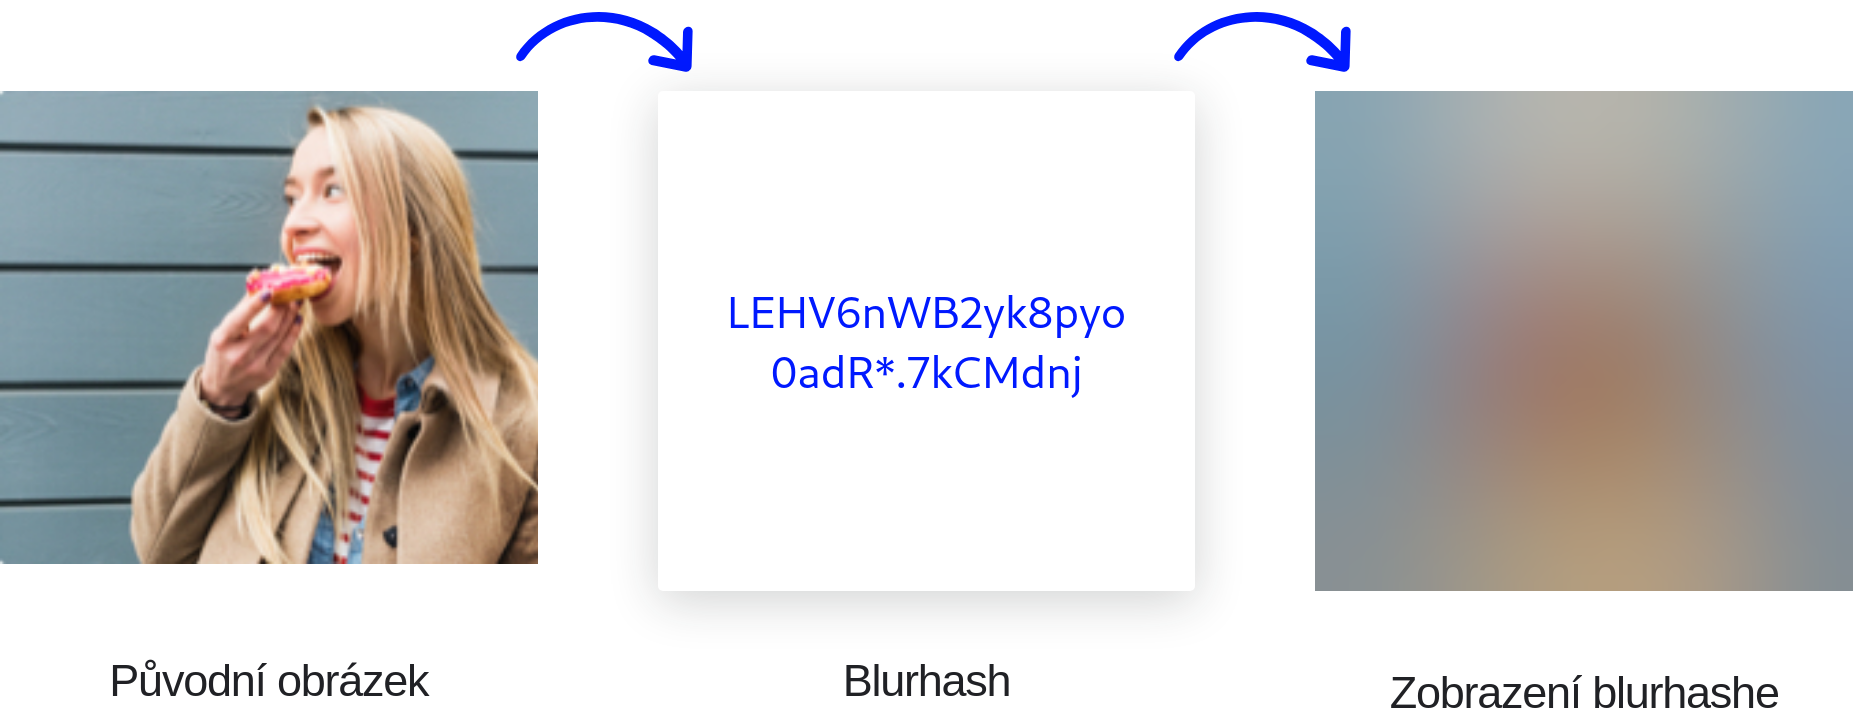
\includegraphics[width=0.8\textwidth]{images/blurhash.png}
	\caption{Generování a zobrazení blurhashe z původního obrázku}
\end{figure}
	
\section{Historický datum příspěvku}\label{section:historical_date}
Každý příspěvek má datum kdy byl vytvořen a historické datum. Historické datum je datum kdy byla fotografie u příspěvku pořízena (z pravidla starší data). U takto starých dat je nutné počítat s tím že se může jedna pouze o odhad, proto není možné použít datum ve formátu podle standartu ISO 8601 jak je zvykem. V autorem navržené struktuře se počítá s tím, že je znám alespoň rok, jako dodatečné informace lze přidat i měsíc, případně den. Zároveň se ale může jednat o určité časové období (například červen až červenec roku 1984), proto jsou vlastnosti rozděleny na počáteční a konečné datum. V případě že se o období nejedná, jsou počáteční a konečné datum stejné. V praxi jde o šest vlastnosí, které má každý příspěvek: startDay, startMonth, startYear, endDay, endMonth, endYear.

\section{Mapa}
    Pro zobrazení mapy je použit balíček react-map-gl, který umožňuje zobrazování např. bodů, polygonů a 3D terénu. Pro zobrazení konkrétních stylů mapy je použit tiling service. Mapa je rozdělena do mřížky ve které jedno pole je jeden tzv. tile, pro tile je poté ze serveru poslán obrázek na kterém je konkrétní část mapy (existují i varianty které používají místo obrázků vektorovou grafiku, což zvyšuje rychlost načítání, a eliminuje efekt rozmatanosti), výhodou je že se ze serveru posílá několik tilů zároveň a ty se poté cachují u klienta. Díky tomu není nutné stahovat data pro jednu část mapy vícekrát. V projektu byl jako tiling service použit Mapbox, jedná se o placené řešení s možností použití předvytvořených stylů mapy, nebo vytvoření stylu zcela vlastního. Alternativou je např. Leaflet, který je poháněn open-source projektem open street maps, který ale obsahuje pouze několik stylů bez možnosti vlastní úpravy.
    \subsection{Geolokace klienta} Pokud nejsou v parametrech URL adresy souřadnice, které mají být zobrazeny, script si vyžádá povolení přístupu k geolokaci. Pokud je přístup povolen, automaticky je lokace mapy nastaven na souřadnice poskytnuté prohlížečem.
    \subsection{Souřadnice v URL adrese}
    Při každém pohybu po mapě jsou souřadnice středu uloženy do paramterů URL adresy. Díky tomu je při obnovení stránky pozice mapy zůstane nezměněna. Toto také umožňuje sdílet konkrétní lokaci na mapě pouze sdílením URL adresy.
    \subsection{Dotazy na server}
    Při změně pohybu mapy je na server odeslán dotaz na všechna místa, které se nacházejí v zobrazené oblasti. Pro zamezení přenosu zbytečných dat dotaz obsahuje seznam míst, která již byla fetchnuta a nacházejí se v dané oblasti, tato místa jsou vynechána z odpovědi serveru.
    \subsection{Seskupování bodů}
    Místa na mapě jsou zobrazena jako ikony s fotografií místa. Pokud by bylo mnoho bodů na malém prostoru, mohly by se nevzájem překrývat, snižovat přehlednost a zpomalovat pohyb po mapě. Proto je použit tzv. clustering (shlukování více bodů), místo těchto bodů je pak vykreslen pouze jeden, který se nachází na souřadnicích rovnajících se průměru souřadnic všech bodů, které cluster obsahuje. Pro rozhodnutí, který obrázek bude na mapě použit jako ikona jsou porovnány vzdálenosti všech bodů v clusteru od středu clusteru, a jako náhled je použit náhled místa, které je nejblíže středu clusteru. V pravém vrchním rohu ikony je poté číslo vyjadřující počet míst seskupených v clusteru.

\begin{figure}[h]
	\centering
	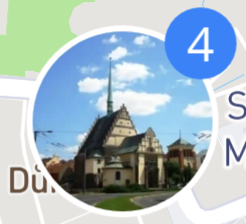
\includegraphics[width=4cm]{images/places_cluster.png}
	\caption{Zobrazení seskupení několika míst na mapě}
\end{figure}
\begin{figure}[h]
	\centering
	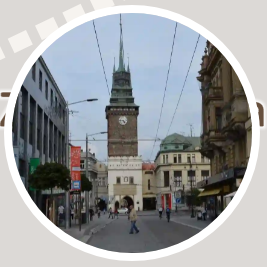
\includegraphics[width=4cm]{images/place.png}
	\caption{Zobrazení jednoho místa na mapě}
\end{figure}

\begin{figure}[h]
	\centering
	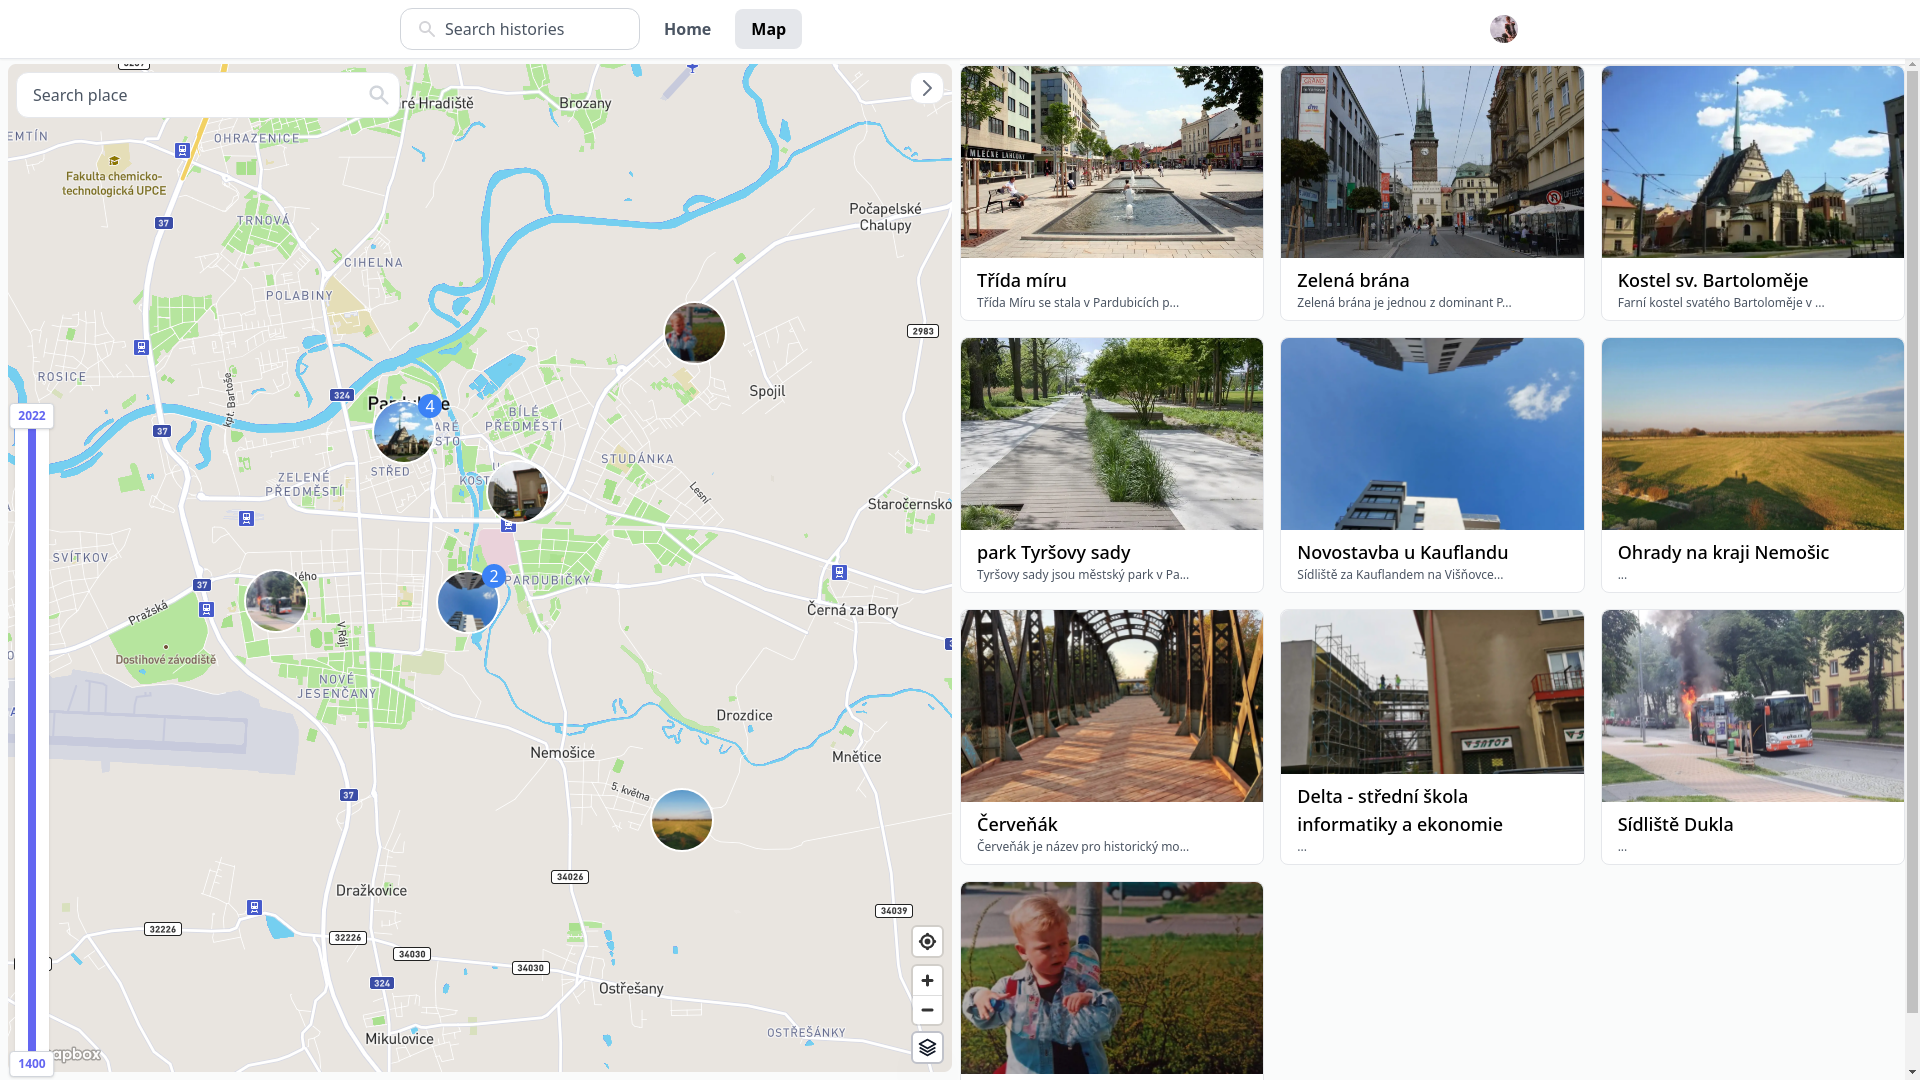
\includegraphics[width=0.8\textwidth]{images/map_page.png}
	\caption{Stránka s mapou}
\end{figure}

\chapter{Zprovoznění}
\section{Docker}
Docker je soubor platforem a služeb poskytujících virtualizaci na úrovni operačního systému pro spouštění softwaru v balíčcích nazývané kontejnery. Docker zajišťuje že programy a aplikace vždy poběží ve stejném prostředí nezávisle na zařízení nebo operačním systému. Jednoduchost spuštění kontejneru usnadňuje nasazení aplikace na server. Celý projekt včetně databáze a úložiště je pak možné spustit jedním skriptem bez nutnosti nastavování.

\chapter{Vývoj}
\section{Verzování}
Git je software pro sledování změn v souborech, které jsou součástí repozitáře. Git poskytuje možnost se kdykoliv vrátit do jakékoliv verze projektu. Git lze také použít při kolaboraci více programátorů, nebo pro synchronizaci kódu.
\section{Testování}
\subsection{Při vývoji}  
\paragraph{Unit testing} je automatizované testování jednotlivých funkcí kódu zadáním vstupních parametrů a následným porovnání výsledků s očekávanými výsledky.
\paragraph{Linter} je označení pro skupinu nástrojů, analyzující statický kód bez nutnosti jeho spuštění. Zároveň zajišťuje jednostnost kódu kontrolou pravidel pro formátování. 
\subsubsection{Nahlašování vzniklých chyb}
\paragraph{Sentry}


 

\section{CI/CD}
\subsection{Aktualizace knihoven}
\subsection{Kontrola zranitelností}
\subsection{Github actions} 


%% Citace
\begin{thebibliography}{100}

    \bibitem{NSFW} NSFW Meaning, what does NSFW mean in text \textit{myenglishteacher.eu} [online]. [cit. 2022-03-19]. Dostupné z: \url{https://www.myenglishteacher.eu/blog/nsfw-meaning/}
    
    \bibitem{GarbageCollection} The Very Basics of Garbage Collection \textit{basen\.oru\.se} [online]. [cit. 2022-03-19]. Dostupné z: \url{http://basen.oru.se/kurser/koi/2008-2009-p1/texter/gc/index.html/}
    
    \bibitem{whatIsRuntimeEnvironment} What Does Runtime Environment (RTE) Mean \textit{Techopedia} [online]. [cit. 2022-03-19]. Dostupné z: \\ \url{https://www.techopedia.com/definition/5466/runtime-environment-rte}
    
    \bibitem{PardubiceVBehuCasuFB} Zajímavosti, videa a obrázky z historie Pardubic \textit{Pardubice v běhu času} [online]. [cit. 2022-03-19]. Dostupné z: \url{https://www.facebook.com/groups/starepardubice/}
    
    \bibitem{DynamicVsStaticTyping} Dynamic typing vs. static typing \textit{Oracle docs} [online]. [cit. 2022-03-19]. Dostupné z: \\ \url{https://docs.oracle.com/cd/E57471_01/bigData.100/extensions_bdd/src/cext_transform_typing.html}
    
    \bibitem{whatIsTypescript} What is typescript \textit{typescripttutorial.net} [online]. [cit. 2022-03-19]. Dostupné z: \url{https://www.typescripttutorial.net/typescript-tutorial/what-is-typescript/}
    
    \bibitem{typescriptForTheNewProgrammer} TypeScript for the New Programmer \textit{Typescript docs} [online]. [cit. 2022-03-19]. Dostupné z: \url{https://www.typescriptlang.org/docs/handbook/typescript-from-scratch.html/}
    
    \bibitem{whatIsNpmW3} What is npm \textit{W3 schools} [online]. [cit. 2022-03-19]. Dostupné z: \url{https://www.w3schools.com/whatis/whatis_npm.asp}
    
    \bibitem{aboutNpm} About npm \textit{NPM docs} [online]. [cit. 2022-03-19]. Dostupné z: \url{https://docs.npmjs.com/about-npm}
    
    \bibitem{graphqlIntroduction} Introduction to GraphQL \textit{GraphQL} [online]. [cit. 2022-03-19]. Dostupné z: \url{https://graphql.org/learn/}
    
    \bibitem{graphqlTypes} Schemas and Types \textit{GraphQL} [online]. [cit. 2022-03-19]. Dostupné z: \url{https://graphql.org/learn/schema/#type-system}
    
    \bibitem{restApiRedHat} What is REST API? \textit{Red Hat} [online]. [cit. 2022-03-19]. Dostupné z: \url{https://www.redhat.com/en/topics/api/what-is-a-rest-api/}
    
    \bibitem{whatIsApiAws} What is an API? \textit{Amazon AWS} [online]. [cit. 2022-03-19]. Dostupné z: \url{https://aws.amazon.com/what-is/api/}
    
    \bibitem{whatIsFrontend} Frontend vs. backend: what's the difference? \textit{Pluralsight} [online]. [cit. 2022-03-19]. Dostupné z: \url{https://www.pluralsight.com/blog/software-development/front-end-vs-back-end/T}
    
    \bibitem{reactComponentsAndProps} Components and Props \textit{React docs} [online]. [cit. 2022-03-19]. Dostupné z: \url{https://reactjs.org/docs/components-and-props.html}
    
    \bibitem{gettingStartedReact} Getting started \textit{React docs} [online]. [cit. 2022-03-19]. Dostupné z: \url{https://reactjs.org/docs/getting-started.html}
    
    \bibitem{whatIsSSR} Client-side vs. server-side rendering \textit{Free code camp} [online]. [cit. 2022-03-19]. Dostupné z: \url{https://www.freecodecamp.org/news/what-exactly-is-client-side-rendering-and-hows-it-different-from-server-side-rendering-bd5c786b340d/}
    
    \bibitem{whatIsSEO} What Is SEO \textit{Next.js docs} [online]. [cit. 2022-03-19]. Dostupné z: \url{https://moz.com/learn/seo/what-is-seo}
    
    \bibitem{nextGetStarted} Gettings started \textit{Next.js docs} [online]. [cit. 2022-03-19]. Dostupné z: \url{https://nextjs.org/docs/getting-started}
    
    \bibitem{tailwindDocumentation} Get started with Tailwind CSS \textit{Tailwind CSS} [online]. [cit. 2022-03-19]. Dostupné z: \url{https://tailwindcss.com/docs/installation/}
    
    \bibitem{graphqlCodeGeneratorDocs} Introduction to GraphQL Code Generator \textit{GraphQL code generator docs} [online]. [cit. 2022-03-19]. Dostupné z: \url{https://www.graphql-code-generator.com/docs/getting-started}
    
    \bibitem{aboutNodeJS} About Node.js® \textit{Node.js®} [online]. [cit. 2022-03-19]. Dostupné z: \url{https://nodejs.org/en/about/}
    
    \bibitem{IPFSDocs} IPFS is a distributed system for storing and accessing files, websites, applications, and data \textit{IPFS} [online]. [cit. 2022-03-19]. Dostupné z: \url{https://docs.ipfs.io/}
    
    \bibitem{decentralizedVsTrustless} Decentralized vs Trustless Networks \textit{Bluzelle} [online]. [cit. 2022-03-19]. Dostupné z: \url{https://bluzelle.com/blog/decentralized-vs-trustless-networks}
    
    \bibitem{decentralizedAndDistributedNetworks} Centralized, Decentralized, \& Distributed Networks \textit{Cryptopedia} [online]. [cit. 2022-03-19]. Dostupné z: \url{https://www.gemini.com/cryptopedia/blockchain-network-decentralized-distributed-centralized}
    
    \bibitem{decentralizedAndTrustless} Decentralized and Trustless Networks \textit{Hackernoon} [online]. [cit. 2022-03-19]. Dostupné z: \url{https://hackernoon.com/decentralized-and-trustless-networks-f881671fae4e}
    
    \bibitem{IPFScontentAddressing} Content addressing and CIDs \textit{IPFS} [online]. [cit. 2022-03-19]. Dostupné z: \url{https://docs.ipfs.io/concepts/content-addressing/}
    
    \bibitem{IPFSPersistence} Persistence | IPFS Docs \textit{IPFS} [online]. [cit. 2022-03-19]. Dostupné z: \url{https://docs.ipfs.io/concepts/persistence/}
    
    \bibitem{IPFSgateways} IPFS Gateway \textit{IPFS} [online]. [cit. 2022-03-19]. Dostupné z: \url{https://docs.ipfs.io/concepts/ipfs-gateway/}
    
    \bibitem{whatIsS3} What is Amazon S3? \textit{Amazon AWS} [online]. [cit. 2022-03-19]. Dostupné z: \url{https://docs.aws.amazon.com/AmazonS3/latest/userguide/Welcome.html}
    
    \bibitem{whatIsDatabase} What Is a Database? \textit{Oracle} [online]. [cit. 2022-03-19]. Dostupné z: \url{https://www.oracle.com/database/what-is-database/}
    
    \bibitem{whatIsACID} The ACID Database Model \textit{Lifewire} [online]. [cit. 2022-03-19]. Dostupné z: \url{https://www.lifewire.com/the-acid-model-1019731/}
    
    \bibitem{graphenTheorie} Graphentheorie \textit{Mathepedia} [online]. [cit. 2022-03-19]. Dostupné z: \url{https://mathepedia.de/Graphentheorie.html}
    
    \bibitem{graphDatabasesIntroduction} Graph Databases for Beginners: Why Graph Technology Is the Future \textit{Neo4j} [online]. [cit. 2022-03-19]. Dostupné z: \url{https://neo4j.com/blog/why-graph-databases-are-the-future/}
    
    \bibitem{graphAlgorithms} Graph Algorithms in Neo4j: Neo4j Graph Analytics \textit{Neo4j} [online]. [cit. 2022-03-19]. Dostupné z: \url{https://neo4j.com/blog/graph-algorithms-in-neo4j-neo4j-graph-analytics/}
    
    \bibitem{aboutNeo4j} The Fastest Path to Graph \textit{Neo4j} [online]. [cit. 2022-03-19]. Dostupné z: \url{https://neo4j.com}
    
    \bibitem{CypherQL} Cypher Query Language \textit{Neo4j} [online]. [cit. 2022-03-19]. Dostupné z: \url{https://neo4j.com/developer/cypher/}
    
    \bibitem{Neo4jNamingRules} Naming rules and recommendations - Neo4j Cypher Manual \textit{Neo4j} [online]. [cit. 2022-03-19]. Dostupné z: \url{https://neo4j.com/docs/cypher-manual/4.4/syntax/naming/}
    
    \bibitem{Neo4jSparialFunctions} Spatial functions - Neo4j Cypher Manual \textit{Neo4j} [online]. [cit. 2022-03-19]. Dostupné z: \url{https://neo4j.com/docs/cypher-manual/4.4/functions/spatial/}
    
    \bibitem{nextImage} API documentation for the Image Component and Image Optimization \textit{Next.js docs} [online]. [cit. 2022-03-19]. Dostupné z: \url{https://nextjs.org/docs/api-reference/next/image}
    
    \bibitem{blurhash} BlurHash is a compact representation of a placeholder for an image \textit{Blurhash} [online]. [cit. 2022-03-19]. Dostupné z: \url{https://blurha.sh/}
    
    \bibitem{blurhashWoltBlog} How we came to create a new image placeholder algorithm, BlurHash \textit{Wolt blog} [online]. [cit. 2022-03-19]. Dostupné z: \url{https://blog.wolt.com/hq/2019/07/01/how-we-came-to-create-a-new-image-placeholder-algorithm-blurhash/}
    
    \bibitem{blurhashScreenshot} Obrázek převzat z https://blurha.sh \textit{Blurhash} [online]. [cit. 2022-03-19]. Dostupné z: \url{https://blurha.sh/}
    
    \bibitem{reactComponentsAtomicDesign} Atomic Design Methodology \textit{bradfrost.com} [online]. [cit. 2022-03-19]. Dostupné z: \url{https://atomicdesign.bradfrost.com/chapter-2/}
    
    \bibitem{reactComponentsAtomicDesignDiagram} Diagram atomického designu \textit{Github} [online]. [cit. 2022-03-19]. Dostupné z: \url{https://user-images.githubusercontent.com/4838076/33235048-d083dca6-d217-11e7-9aea-9a5ef5ae6fe7.png}
    
    \bibitem{internationalizationVsLocalization} Internationalization vs. localization (i18n vs l10n): What’s the difference? \textit{Lokalise} [online]. [cit. 2022-03-19]. Dostupné z: \url{https://lokalise.com/blog/internationalization-vs-localization/}
    
    \bibitem{whyAreCommentsImportant} Reasons Why Comments Are Important For Instagram \textit{Time square chronicles} [online]. [cit. 2022-03-19]. Dostupné z: \url{https://t2conline.com/reasons-why-comments-are-important-for-instagram/}
    
    
    \bibitem{bootstrap} Build fast, responsive sites with Bootstrap \textit{Bootstrap} [online]. [cit. 2022-03-19]. Dostupné z: \url{https://getbootstrap.com/}
    
    
    \end{thebibliography}
    
    %%%%% CLEAR DOUBLE PAGE!
    \newpage{\pagestyle{empty}\cleardoublepage} 

\end{document}